% Copyright 2023 Andy Casey (Monash) and friends
% TeX magic by David Hogg (NYU)

\documentclass[modern]{aastex631}
\usepackage[utf8]{inputenc}
\usepackage{amsmath}
\usepackage{MnSymbol}

\renewcommand{\twocolumngrid}{}
\addtolength{\topmargin}{-0.35in}
\addtolength{\textheight}{0.6in}
\setlength{\parindent}{3.5ex}
\renewcommand{\paragraph}[1]{\medskip\par\noindent\textbf{#1}~---}

% figure setup
\usepackage{graphicx}
\usepackage{xcolor}
\usepackage[framemethod=tikz]{mdframed}
\usetikzlibrary{shadows}
\definecolor{captiongray}{HTML}{555555}
\mdfsetup{%
innertopmargin=2ex,
innerbottommargin=1.8ex,
linecolor=captiongray,
linewidth=0.5pt,
roundcorner=1pt,
shadow=false,
}
\newlength{\figurewidth}
\setlength{\figurewidth}{0.75\textwidth}

\newcommand{\norm}[1]{\left\lVert#1\right\rVert}

% Other possible titles

% TODO
% [ ] Talk about BOSZ spectra and how the model was constructed.
% [ ] Talk about how we constructed the telluric basis vectors
% [ ] Flesh out discussion points
% [ ] Data section
% -> Blaze???
% [ ] Results section
% -> ON a set of OBAFGKM stars, provides clean and consistent normalisation across these types
% -> ARE WE USING THE NIGHTLY BLAZE?
% -> discuss for alf Cen A, how we selected spectra to get a uniform sampling in SNR, and how we fit them
% -> how we define the consistency measure

% [ ] discussion
% -> We fix vsini / v_rel from the literature, but these can be computed 
% -> 

% text macros
%\newcommand{\chosentitle}{Constrained linear models for stellar spectroscopy}
%\newcommand{\chosentitle}{Constrained linear absorption models for stellar spectroscopy}
%\newcommand{\chosentitle}{The Unreasonable Effectiveness of Linear Models in Stellar Spectroscopy}
%\newcommand{\chosentitle}{Stellar continuum modelling}
\newcommand{\chosentitle}{Constrained linear models for stellar spectroscopy}

\shorttitle{\chosentitle}
\shortauthors{Casey}
\newcommand{\documentname}{\textsl{Article}}
\newcommand{\sectionname}{Section}

\newcommand{\project}[1]{\textit{#1}}
\renewcommand{\vec}[1]{\mathbf{#1}}
\newcommand{\vectheta}{\boldsymbol{\theta}}
\newcommand{\vecalpha}{\boldsymbol{\alpha}}
\newcommand{\vecbeta}{\boldsymbol{\beta}}
\newcommand{\vecgamma}{\boldsymbol{\gamma}}
\newcommand{\vecW}{\mathbf{W}} % stellar line absorption basis weights
\newcommand{\vecF}{\mathbf{F}} % stellar line absorption basis vectors
\newcommand{\vecG}{\mathbf{G}} % telluric line absorption basis vectors
\newcommand{\vecH}{\mathbf{H}} % continuum basis vectors
\newcommand{\vecX}{\mathbf{X}}


\newcommand{\hadamard}{\odot}
\newcommand{\apogee}{\project{APOGEE}}
\newcommand{\boss}{\project{BOSS}}
\newcommand{\sdss}{\project{SDSS}}
\newcommand{\eso}{\project{ESO}}
\newcommand{\harps}{\project{HARPS}}

% math macros
\newcommand{\unit}[1]{\mathrm{#1}}
\newcommand{\mps}{\unit{m\,s^{-1}}}
\newcommand{\kmps}{\unit{km\,s^{-1}}}
\newcommand*{\transpose}{^{\mkern-1.5mu\mathsf{T}}}
%\newcommand{\transpose}{^\mathsf{T}}



% notes
\definecolor{tab:blue}{HTML}{1170aa}
\definecolor{tab:red}{HTML}{d1615d}
\newcommand{\todo}[1]{\textcolor{tab:red}{#1}}

\sloppy\sloppypar\raggedbottom\frenchspacing
\begin{document}

\title{\chosentitle}

\author[0000-0003-0174-0564]{Andrew R. Casey}
\affiliation{School of Physics \& Astronomy, Monash University, Australia}
\affiliation{Centre of Excellence for Astrophysics in Three Dimensions (ASTRO-3D)}
\affiliation{Center for Computational Astrophysics, Flatiron Institute, a division of the Simons Foundation}

\author{friends}
%\author[0000-0003-2866-9403]{David W. Hogg}
%\affiliation{Center for Cosmology and Particle Physics, Department of Physics, New York University}
%\affiliation{Max-Planck-Institut f\"ur Astronomie, Heidelberg}
%\affiliation{Center for Computational Astrophysics, Flatiron Institute, a division of the Simons Foundation}

% Other people who will be invited as co-authors (non-exhaustive list):
%   Holtzman, Wheeler, Sayjdari, Bedell, Dream team, Astra folks, CCA data group


\begin{abstract}\noindent
Forward modelling stellar spectra usually requires a spectral synthesis code, or some non-linear interpolator constructed from a curated training set.
These approaches require pre-processing steps (e.g., continuum rectification) which, when performed separately, can bias subsequent measurements.
Here we present a \emph{linear} model that simultaneously fits stellar absorption, telluric transmission, and the joint continuum-instrument response.
Stellar absorption and telluric transmission are each modelled by factorizing a grid of rectified theoretical spectra into two non-negative matrices: basis weights and basis vectors.
The non-negativity constraint ensures that basis vectors are strictly additive.
The joint continuum-instrument response is modelled with a Fourier basis. 
Together this set of bases represents a very effective linear model for stellar spectroscopy, where the linearity ensures that inference is convex, stable, and fast.
This model allows us to reliably fit nuisance parameters (e.g., tellurics, continuum, radial velocity, rotational or macroscopic broadening), without any prior knowledge about the fundamental stellar properties.
We demonstrate our method by fitting \todo{toy models of M-dwarf spectra where we recover the correct continuum, and by fitting} \eso/\harps\ high-resolution echelle spectra of OBAFGKM-type stars.
From repeat observations of $\alpha$-Centauri A we show that our approach yields continuum estimates that are consistent to 0.2\% at S/N $\sim$ 100, and better than 0.5\% at S/N $\sim$ 30.
\end{abstract}

% for S/N > 100, 1-sigma scatter is 0.22%
% for S/N > 50, 1-sigma scatter is 0.35%
% for S/N > 30, 1-sigma scatter is 0.46%

\keywords{Some --- keywords --- here}

\section*{}\clearpage
\section{Introduction}\label{sec:intro}

Continuum normalization\footnote{Or continuum rectification, as it was historically described.} is often required before estimating stellar parameters and chemical abundances, because these quantities are inferred from line strengths measured \emph{relative} to the continuum.
The practicalities of continuum rectification is ripe with subjectivity, for justified historical reasons: often a consistent procedure is more useful than an abstract one, so people tend to stick with what they know. While there is general agreement in the literature that consistent continuum normalization is important, there is no apparent consensus on how it should be done.\\

There is a variety of rectification strategies used to achieve different goals. Classical spectroscopists might make some coarse estimate of the continuum for the spectrum, and locally refine the continuum for each sbsorption line of interest. This process is often done by hand,\footnote{Albeit they are often experienced hands. See \citet{Bensby:2014}: \quote{`\emph{more than 300\,000 equivalent widths were measured by (the first author's right) hand}'}.} although some graphical user interface tools exist to streamline the process and improve reproducibility. This approach usually restricts the spectroscopist to only measuring strengths of isolated lines: those that are not blended by neighbouring atomic lines or strong molecular bands. In contrast, industrial spectroscopists have a different objective: one where they solely for a \emph{consistent} continuum normalization procedure. For them the process does not have to deliver the true continuum, but it should deliver a \emph{pseudo}-continuum that is consistent for stars of similar stellar parameters and signal-to-noise (S/N) ratios.\\

Fitting the continuum correctly requires you to know where there is absorption. But knowing where there is line absorption requires you to (at least) know the stellar parameters. Without knowing the stellar parameters -- or having a good model for line absorption -- spectroscopists have developed various bespoke methods. A popular choice is to iteratively mask pixels in an asymmetric manner (so-called `sigma clipping') to exclude data points some chosen level below the current estimate of the continuum. This works well if the practictioner can confidently set the bounds on where to exclude data. However, those parameters would need to be different for a more metal-rich star, or for a spectrum with a low signal-to-noise (S/N) ratio. Exactly how to specify the asymmetric clipping parameters comes down to experience.\\

An alternative is simply to mask all pixels except a carefully selected set of so-called `continuum pixels'. This is painstaking work to perform manually, but can be done by iteratively training data-driven models, or building masks from approximate line strengths computed from atomic properties. In either scenario, the set of continuum pixels is only valid for stars of a similar type and metallicity. In many cases, there are simply \emph{no} continuum pixels (e.g., near a molecular absorption band in an M-dwarf), and the best we can compute is a \emph{pseudo}-continuum.\\

A variety of methods for rectifying spectra are described in the literature. \todo{Some summary of those. Includes the rolling ball thing, RASSINE, and any others?}\\


In an ideal scenario the continuum is jointly fit with the stellar parameters. Unfortunately, predicting the emergent spectrum is usually expensive. In Section~\ref{sec:methods} we describe a family of methods to address these problems.
The methods we describe use non-negative matrix factorization (NMF) to approximate line absorption. NMF is a linear model to describe large non-negative matrix by two smaller matrices, both with non-negative elements. This non-negativity provides a very useful constraint that is applicable in many areas of astronomy (i.e., where things cannot physically be negative), but NMF has seen relatively little use in astronomy compared to other research areas, or other dimensionality reduction techniques.
We discuss limitations and potential extensions of our work in Section~\ref{sec:discussion}, before concluding in Section~\ref{sec:conclusions}.\\

%The typical analysis procedure for this kind of spectra might involve selecting (by hand) pixels that do not appear to be obviously affected by line (or molecular) absorption, and fitting a smooth function to represent the continuum. This process would be repeated per-order, often ignoring the selection of pixels in the previous order (which overlaps in wavelength). A subsequent local continuum determination would be made for each line.


\section{Methods}\label{sec:methods}

We will assume a forward model that includes three components: one that represents continuum-normalized stellar absorption (e.g., molecular or atomic line absorption); a second to describe telluric transmission; and a third to represent the smooth continuum.\footnote{Throughout this paper when we refer to the continuum, we mean the joint continuum-instrument response. These are different things that enter multiplicatively, but cannot be disentangled without extra work.} We will require all components to be linear models, which ensures that inference is stable and fast. In practice the linear models we construct seem sufficient to model stellar spectra for the purposes of continuum normalization and handling other nuisances.\\

% TODO: list explicit assumptions with hogg in person

Here we will describe the method in general before outlining the implementation details. We assume the data are a one-dimensional spectrum with $P$ pixels, where the $i$-th pixel has wavelength $\lambda_i$, flux $y_i$, and flux error $\sigma_{y_i}$ (with $1 \leq i \leq P$). The forward model for the flux in the $i$-th pixel can be expressed as the element-wise (Hadamard; $\hadamard$) multiplication of what we will describe as the stellar absorption model $f(\lambda_i; \vecalpha)$, the telluric transmission model $g(\lambda_i; \vecbeta)$, and the continuum-instrument response model $h(\lambda_i;\vecgamma)$
\begin{align}
    y_i &= f(\lambda_i;\vecalpha)\hadamard{}g(\lambda_i;\vecbeta)\hadamard{}h(\lambda_i;\vecgamma) + \mbox{noise}
\end{align}
where the components $f(...)$, $g(...)$, and $h(...)$ are defined below. Throughout this paper we fit in (natural) log-transformed data space $\vec{Y} = \log{\vec{y}}$ with the transformed variance in the $i$-th pixel
\begin{eqnarray}
    \vec{C}_{ii} = \left(\frac{\sigma_{y,i}}{y_i} - \frac{\sigma_{y,i}^2}{2y_i^2} + \frac{2\sigma_{y,i}^3}{8y_i^3} - \frac{6\sigma_{y,i}^4}{24y_i^4}\right)^2
\end{eqnarray}
\noindent{}computed by taking a swiftly Taylor series expansion. The log-transformation changes the element-wise product into a convenient summation:
\begin{align}
    \label{eq:log_y}
    \vec{Y} &= \log{f(\vec{\lambda}; \vecalpha)} + \log{g(\vec{\lambda};\vecbeta)} + \log{h(\vec{\lambda};\vecgamma)} \quad .
\end{align}\\

We now turn to defining each model component in detail.
The stellar absorption model $f(\lambda_i;\vecalpha)$ predicts the rectified stellar line absorption at wavelength $\lambda_i$ given parameters $\vecalpha$. We construct the line absorption model $f(\lambda_i;\vecalpha)$ from a set of $N$ continuum-normalized theoretical spectra (each with $D$ fluxes) using non-negative matrix factorization (NMF).
The theoretical spectra used to construct the line absorption model do not have to have the same wavelength sampling and instrument line spread profile as the data, but at inference time there is a need to interpolate (or evaluate) the line absorption model to the $P$ observed wavelengths.\\

We refer to our $N \times D$ matrix of continuum-rectified theoretical stellar spectra as $\vec{S}$. This is a dense matrix: there are no entries of exactly zero, with many entries near 1 (no absorption). However, a small transformation to this matrix makes it extremely sparse. Numerous transformations are possible\footnote{Another sparse transformation is $1 - \vec{M}$, but this makes our resulting model non-linear.}, but for many reasons we chose to factorize the negative logarithm of $\vec{S}$ into two smaller matrices $\vec{W}_\star$ and $\vec{F}$ such that,
\begin{eqnarray}
    \label{eq:nmf}
    -\log\left({\vec{S}}\right) \approx \vec{W}_\star\transpose\vec{F}
\end{eqnarray}
where $\vec{W}_\star$\footnote{The star in $\vec{W}_\star$ differentiates it from the basis weights found from factorizing telluric spectra $\vec{W}_\earth$.} is a $K \times N$ matrix of \emph{basis weights}, where $K$ is the number of chosen basis vectors, and $\vec{F}$ is a $K \times D$ matrix of NMF \emph{basis vectors}. The factorization of $-\log{\vec{S}}$ into $\vec{W}_\star\transpose\vec{F}$ requires that all elements in $-\log\left({\vec{S}}\right)$, $\vec{W}_\star$, and $\vec{F}$ be non-negative. The number of basis components $K$ should be significantly smaller than both the number of input spectra $N$ and the number of pixels $D$ per spectrum.\\%Figure~\ref{fig:schematic} illustrates some example basis vectors factorized from theoretical spectra in the \apogee\ wavelength range.\\


%on previous works on NMF and data analysis more broadly. We would like the naming conventions to be consistent with those papers, but this nomenclature is easily overloaded. For this reason, we make clear definitions: throughout this paper we will refer to $\vecW$ as the NMF \emph{basis weights} and $\vecH$ as the NMF \emph{basis vectors}. \\


%Here $\vec{W}$ is a $N \times C$ matrix that can be thought of as $C$ basis weights per spectrum, and $\vec{H}$ is a $C \times D$ matrix of $C$ corresponding basis vectors each with $D$ pixels.

%The nomenclature  draws on previous works on NMF and data analysis, but this nomenclature is easy to overload, so throughout this paper we will refer to $\vecW$ as the NMF \emph{basis weights}, $\vecalpha$ as the NMF \emph{basis coefficients}, $\vecH$ as the NMF \emph{basis vectors}, and $\vectheta$ (not yet defined) will refer to the amplitudes of the sine-and-cosine basis.

The factorization of $-\log\left({\vec{S}}\right)$ into $\vec{W}_\star\transpose\vec{F}$ is reasonably fast and easy to compute given existing packages in modern programming languages. In general we found substantial improvements by initializing $\vec{F}$ with non-negative double singular value decomposition, where zeros were filled-in with the average of $-\log\left({\vec{S}}\right)$: this is the default behaviour in many packages. We found that factorizing $\vec{W}_\star\transpose\vec{F}$ by coordinate descent was substantially faster than using multiplicative updates, \todo{until reaching a plateau in reconstruction error, at which point we would iterate further using multiplicative updates.} The multiplicative update rules are appealing because they are convex, do not require many choices, and they can be efficiently iterated on a graphics card.\\


There are very few requirements of the theoretical spectral grid. There are no requirements on the number of dimensions (e.g., whether or not to include $[\alpha/\mathrm{Fe}]$, $[\mathrm{C/Fe}]$), and no strict requirements (see Section~\ref{sec:discussion}) on spacing in between points. The only implicit requirement is that the theoretical spectra should approximately span the range of stars that you intend to fit. This is more of a recommendation than a requirement: in practice we found that a grid trained on theoretical spectra of A- to M-type stars was also sufficiently flexible to model many O-type stars. For these reasons, we chose to include as many theoretical spectra as our memory constraints would allow.\footnote{If the number of spectra exceeds your memory constraints then there are numerous strategies available: you can use memory-mapped arrays, use lower precision float types, compute updates in batches, or simply skip every $n$th spectrum.}\\

We used the BOSZ spectral grid to construct basis vectors for a stellar line absorption model. This is a high-resolution ($\mathcal{R} \sim 300{,}000$) finely sampled theoretical grid computed using the \project{ATLAS9} code with \project{MARCS} models atmospheres. The grid spans a reasonably large range in stellar parameters, covers the complete wavelength range of the \eso/\harps\ instrument, and importantly it includes the theoretical continuum for each spectrum. We constructed a sparse kernel to convolve the rectified flux to the \eso/\harps\ spectral resolution of $\mathcal{R} \sim 115{,}000$, truncated the convolved spectra between 300-700\,nm, and clipped any rectified flux values exceeding 1 (e.g., emission lines) as they violate our NMF requirements. The matrix $\vec{S}$ includes all \todo{X} convolved BOSZ spectra, with \todo{N} pixels each, which we randomly shuffled before factorization. We then factorized this matrix into $K = 16$ basis vectors by coordinate descent for \todo{10,000} steps, \todo{and then X steps using multiplicative updates}. After training, the Frobenius loss, also known as the L2 reconstruction loss
\begin{eqnarray}
    L_2 = \norm{{\left(-\log{\vec{S}}\right) - \vec{W}_\star\transpose\vec{F}}}^2
\end{eqnarray}
\noindent{}was found to be \todo{X}. Figure~\ref{fig:schematic} shows some example basis vectors computed by this factorization, where it is somewhat striking that the basis vectors are identifiable by astrophysical mechanism, since no stellar parameters (or astrophysics of any kind) are included in the factorization process. For example, one basis vector just includes hydrogen lines. Another basis vector only has CO-molecule lines. We expand on this observation in later sections.\\

\begin{figure*}
    \includegraphics*[width=\textwidth]{nmf_plot.pdf}
    \caption{A schematic showing some basis vectors computed by non-negative matrix factorization from a grid of theoretical stellar spectra. \todo{Update this for BOSZ spectra, not APOGEE.}\label{fig:schematic}}
\end{figure*}


\noindent{}With the non-negative matrix $\vec{F}$ we can now define the logarithm of stellar line absorption function $\log{f(\lambda_i;\vecalpha)}$, which follows from equations~\ref{eq:log_y} and \ref{eq:nmf},
\begin{align}
    \log{f(\lambda_i;\vecalpha)} = -\vec{F}\transpose\vecalpha \label{eq:log-f}
\end{align}
where $\vecalpha \in [0, \infty)$ is a column vector of $K$ \emph{stellar basis weights} to be solved at inference time. Here, $\vecalpha$ is analogous to a column in $\vecW_\star$: it represents the $K$ weights needed to reconstruct the stellar absorption from the $K$ basis vectors $\vec{F}$. Note that because $\vecalpha$ and $\vec{F}$ are both restricted to have non-negative elements, this severely restricts the flexibility of $f(...)$, leaving $h(...)$ to represent the smooth continuum-instrument response. \\

Telluric transmission can be included in a similar way to stellar absorption. We used a grid of model telluric transmission spectra computed for the \texttt{PypeIt} project. These spectra are computed using the Line-by-Line Radiative transfer Model for an array of observatory locations (latitude, longitude) and atmospheric temperatures, pressures, humidity, and airmass. The original grid of telluric transmission spectra was not available to us. Instead, we used a representation of this grid that is shipped with \texttt{PypeIt}, and compressed using Principal Component Analysis and an inverse hyperbolic sine transformation, to approximate the original grid. With this reconstructed grid, we factorized the negative log of theoretical telluric absorption 
\begin{eqnarray}
    -\log\vec{M} \approx \vec{W}\transpose_\earth\vec{G}
\end{eqnarray}
\noindent{}into two-non negative matrices $\vec{W}\transpose_\earth$ and $\vec{G}$ using $L = 4$ basis vectors. We took \todo{10,000} iterations using coordinate descent, at which point the reconstruction loss was \todo{X}. With the non-negative matrix $\vec{G}$, the function $\log{g\left(\lambda_i;\vecbeta\right)}$ is simply
\begin{eqnarray}
    \log{g(\lambda_i;\vecbeta)} = -\vec{G}\transpose\vecbeta
\end{eqnarray}
where $\vecbeta \in [0, \infty)$ is column vector of $L$ \emph{telluric basis weights} in to be solved at inference time. 
%We could restrict $\vecbeta \in [0, \max(\vec{W}_\earth)]$, and $\vecalpha \in [0, \max(\vec{W}_\star)]$, but in practice this is not necessary, and a more flexible approach might be to apply a feature weighting prior (see Section~\todo{?}). 
Like $\vecalpha$, $\vecbeta$ is analogous to a column in $\vec{W}_\earth$: it represents the $L$ basis weights needed to reconstruct the telluric absorption.\\

There are many suitable choices for the logarithm of the continuum-instrument response model $\log{h(\lambda_i;\vecgamma)}$. Here we chose a Fourier basis of sine and cosine functions because it is a linear representation, and is sufficiently flexible for modelling the joint continuum-instrument response across a variety of spectrographs. The component $\log{h(\lambda_i;\vecgamma)}$ is expressed compactly as
\begin{align}
    \log{h(\lambda_i;\vecgamma)} = \vec{H}\vecgamma
\end{align}
where $\vec{H}$ is a design matrix where the elements of the $j$th column are, % todo: shape of design matrix
\begin{align}
    \vec{H}_{j}(\lambda_i) & = \left\{\begin{array}{cl}\displaystyle\cos\left(\frac{\pi\,[j-1]}{P}\,\lambda_i\right) & \mbox{for $j$ odd} \\[3ex]
    \displaystyle\sin\left(\frac{\pi\,j}{P}\,\lambda_i\right) & \mbox{for $j$ even}\end{array}\right. ~,
\end{align}
\noindent{}where $P$ is a length scale which we set to be twice the length of the wavelength range to fit (e.g., twice the peak-to-peak range of an echelle order). %The design matrix $\vec{H}$ can be constructed \emph{a priori} ibce before inference begins. 
Throughout this paper we will describe $\vecgamma$ as the sine-and-cosine \emph{coefficients}.\\

\noindent{}With $f(\lambda_i;\vecalpha)$, $g(\lambda_i;\vecbeta)$ and $h(\lambda_i;\vecgamma)$ now defined, we can expand the forward model for the log-transformed data $\vec{Y}$,
\begin{equation}
    \vec{Y} = -\vec{F}\transpose\vecalpha - \vec{G}\transpose\vecbeta + \vec{H}\vecgamma
\end{equation}
\noindent{}which we can compactly write as
\begin{equation}
    \vec{Y} = \vec{A}\vec{X}
\end{equation}
where the parameters and design matrices are stacked to construct $\vec{A}$ and $\vec{X}$:
\begin{eqnarray}
    \vec{A} = \begin{bmatrix}-\vec{F}\transpose\\-\vec{G}\transpose\\\vec{H}\end{bmatrix}
    \quad \mbox{and} \quad
    \vec{X} = \begin{bmatrix}\vecalpha\\\vecbeta\\\vecgamma\end{bmatrix} \quad .
\end{eqnarray}


Given some log-transformed observed flux $\vec{Y}$ and associated covariance matrix $\vec{C}$, this reduces to a weighted least-squares problem. This could be solved directly by linear algebra,
\begin{eqnarray}
    \vec{\tilde{X}} = (\vec{A}\transpose\vec{C}^{-1}\vec{A})^{-1}\vec{A}\transpose\vec{C}^{-1}\vec{Y}
\end{eqnarray}
\noindent{}but this solution is not subject to the constraints $\vecalpha \geq 0$ and $\vecbeta \geq 0$. There are a few ways to solve this system subject to the boundary constraints, but the choice is not very important because the problem is convex. For simplicity we use the truncated reflective trust region algorithm where we stop optimizing once the relative tolerance has improved by less than $10^{-16}$.\\


%In later sections we describe some situations where we may want to penalize values of $\vecalpha$. We perform this by feature weighting, which is equivalent to setting a prior on the distribution that $\vecalpha$ can be drawn from. We introduce the feature weighting matrix $\vec{\Lambda}$, where $K$ is the number of basis vectors chosen for NMF and $L$ is the number of Fourier modes. We set the first $K \times K$ elements of $\vec{\Lambda}$ to $\mathrm{Cov}{\left(\vec{W}\vec{W}\transpose\right)}$ and set all other elements of $\vec{\Lambda}$ to zero. We can scale the strength of this feature weighting by a scalar $\lambda$ (\todo{nomenclature overload of lambda}) and solve for the parameters $\vec{\tilde{X}}$ with
%\begin{eqnarray}
%    \vec{\tilde{X}} = (\vec{A}\transpose\vec{C}^{-1}\vec{A} + \lambda\vec{\Lambda})^{-1}\vec{A}\transpose\vec{C}^{-1}\vec{Y} %\quad .
%\end{eqnarray}\\

After solving for $\vec{\tilde{X}}$, the (un-transformed) quantities can be easily computed:
\begin{eqnarray}
    \mathrm{rectified~stellar~flux}, \quad &f& = \exp{\left(-\vec{F}\transpose\boldsymbol{\tilde{\alpha}}\right)} \\
    \mathrm{telluric~transmission},\quad  &g& = \exp{\left(-\vec{G}\transpose\boldsymbol{\tilde{\beta}}\right)} \\
    \mathrm{continuum}, \quad &h& = \exp{\left(\vec{H}\boldsymbol{\tilde{\gamma}}\right)}
\end{eqnarray}


\section{Data} \label{sec:data}

Here we seek demonstrate the effectiveness of our model on high-resolution echelle spectra: a scenario in which there are lots of data, and lots of nuisances. The nuisances (e.g., continuum parameters per order; tellurics) are often fit separately which can bias subsequent inferences, and the large data volume (e.g., $3\times10^6$~pixels per spectrum) can make even the fastest non-linear interpolators untenably slow.\\

We searched the \eso\ data archive and selected a set of stars that span the range of spectral types and evolutionary states observed with the \harps\ instrument. The set include OBAFGKM-type stars, main-sequence stars, and red giant branch stars. This selection is not intended to be complete, but is meant to demonstrate the effectiveness of a single linear model for fitting stars across a range of stellar parameters and evolutionary states. \\

We downloaded a psuedo-random exposure for each star. No explicit cut to ensure a minimum signal-to-noise (SNR) ratio, but in practice most exposures have high SNR. We took the measured radial velocity in the calibration files for each spectrum and the computed Barycentric Earth radial velocity to shift the stellar absorption basis vectors to the observed frame.\\

We modelled the continuum in each echelle order as a set of $\todo{M}$ Fourier modes. With $\todo{\approx{70}}$ echelle orders, $\todo{K}$ stellar basis vectors, and $\todo{L}$ telluric vectors, there are $\todo{400}$ parameters and $\sim3\times10^6$ data points. Without \emph{any prior knowledge of the stellar parameters}, we directly solve the (unconstrained) weighted least-squares system (Equation~\ref{eq:wls}). If the solution is outside the parameter bounds, we optimize from this position using truncated reflective trust region algorithm.\\



\begin{figure*}
    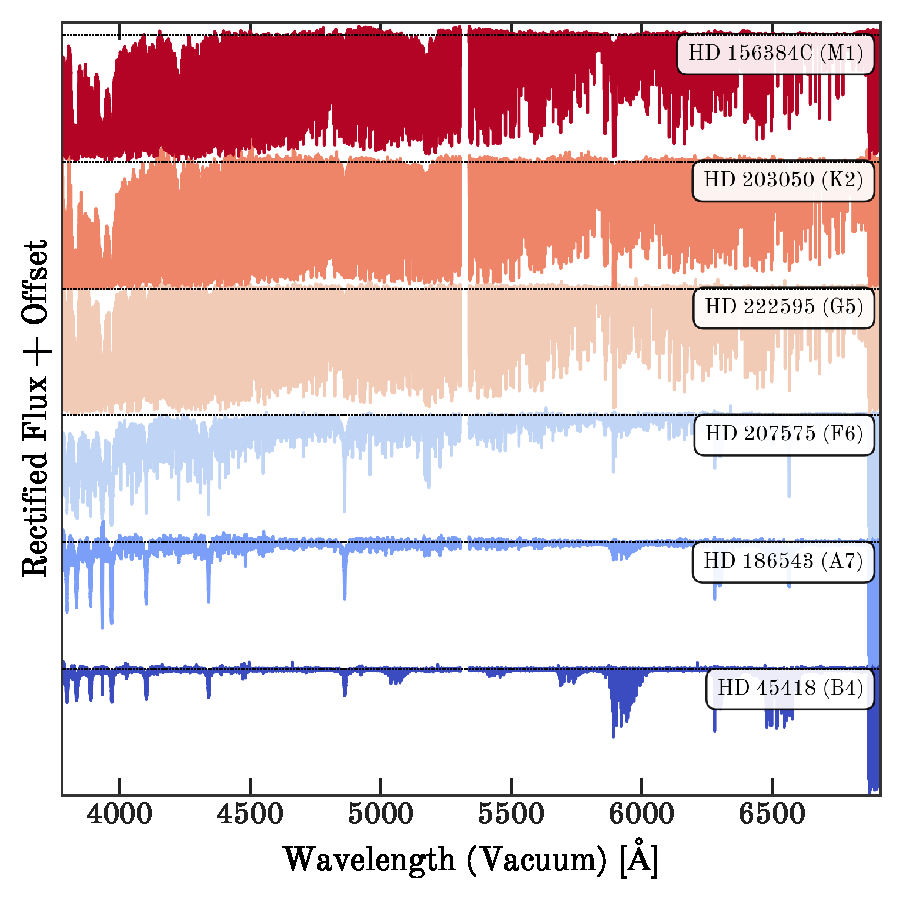
\includegraphics[width=\textwidth, height=\textwidth]{../code/harps_examples.pdf}
    \caption{Continuum-rectified \harps\ spectra of example spectral types from B to M. The model used here includes 16 basis vectors for stellar absorption, and 4 basis vectors for telluric transmission.\label{fig:harps-examples}}
\end{figure*}


\section{Results} \label{sec:results}

We found it usually takes a few core-seconds to fit each exposure ($3\times10^6$~pixels; all echelle orders fit simultaneously). Most of this time is spent constructing the design matrix, which requires (linearly) interpolating the stellar and telluric basis vectors to the observed wavelengths. The fits to each star are partially shown in Figure~\ref{fig:harps-example}. In all cases the data are shown in black, with the stellar absorption model in \todo{red}, telluric transmission in \todo{color}, and continuum in \todo{color}. Overall, the fits to the data are very good, with reduced $\chi^2$ values from \todo{A to B}.\\

In bluer echelle orders, it can be seen that there are no pixels that are true `continuum' pixels (i.e., no absorption). Any continuum normalization method trying to fit these echelle orders would be biased if they did not have a good representation of what stellar spectra look like. \\

Maintaining consistent continuum rectification for low signal-to-noise spectra is challenging. Without a model for stellar spectra or the relative strengths of absorption lines, noisy signals can mimic stellar absorption, causing the continuum to become systematically biased at low signal-to-noise ratios. For this reason, we sought to estimate the consistency of continuum normalization as a function of signal-to-noise ratio.\\

We searched the \eso/\harps/ archive for a star that has been repeatedly observed with a wide range of exposure times, usually because it is the subject of radial velocity asteroseismic monitoring. Through this search we identified alpha Centauri A, which has been observed more than \todo{X} times with \harps. Importantly, there are $\alpha$-Centauri spectra with signal-to-noise ratios of 10, and a nearly even sampling of spectra up to S/N of 300, or even higher (where saturation is visible in the reduced spectra\footnote{Naughty observer.}). We constructed bins of SNR from 0 to 200 in steps of 10. We selected an $\alpha$-Centauri spectrum for every SNR bin interval to provide an even sampling of spectra at low and high SNR. We fit our model to each spectrum, treating it as totally indepdendent from all others.\\

\todo{Now we can see how things behave as a function of SNR.}

\todo{Consistency at low signal-to-noise}
% alf Cen 95th percentile (all wavelengths)
% for S/N > 100, 1-sigma scatter is 0.22%
% for S/N > 50, 1-sigma scatter is 0.35%
% for S/N > 30, 1-sigma scatter is 0.46%

% RASSINE claims 1% (2% in their metric, which is 2 sigma) continuum accuracy of alpha Cen B with HARPS spectra.
% When they exclude bluer than 4500 Angstrom, their continuum accuracy improves to 0.6% (1.2% in their metric)

% If our perormance on alpha Cen A is comparable to theirs on alpha Cen B, then
% our method is about 5x more accurate


%The method can be readily applied to real data once the eigenspectra $\vecH$ have been computed. We experimented with choices of initialisation and inference. Since both components are linear and have closed-form solutions, we did find some success by alternating between solving for $\vecalpha$ and $\vectheta$, but ultimately chose to optimize all parameters $\{\vecalpha,\vectheta\}$ simultaneously. The number of parameters scales as $C + n_\textrm{regions}(2n_\textrm{degree} + 1)$: $C$ amplitudes for $C$ eigenspectra ($\vecalpha$), and $2n_\textrm{degree} + 1$ sine-and-cosine coefficients ($\vectheta$) per chosen continuum region (e.g., per chip). Initializing from small ($10^{-12}$) values of $\vecalpha$ and a closed-form solution of $\vectheta$ (conditioned on small $\vecalpha$) seemed to work well in many scenarios. \\

%In later sections we describe applications of our method to real data. For now we will describe a few options that we found to work reasonably well across all settings, which we have since established as default behaviour in the accompanying software implementation. When faced with the choice of how many spectra to include when performing non-negative matrix factorization, we found good results by including everything that could fit into memory. Using limited precision floats (e.g., float-8) helped. Initialising with non-negative double singular value decomposition (with zeros filled with small random values) seemed to work very well. Multiplicative updates.

% put this in discussion
%As we discuss in Section~\ref{sec:discussion}, this is not true of all linear models: it is a design choice that leads to this strict constraint. Other linear models (e.g., PCA) allow for summation of large positive and negative amplitudes, leading to  of positive and negative eigenspectra,



This is a convex problem that is mathmatically guaranteed to yield the solution that minimizes the $\chi^2$ between the (log-)transformed data and model. However, it does not guarantee that the solution is sensible, or even physically possible. We expand on this in the \emph{Discussion} (Section~\ref{sec:discussion}), but the point here is to highlight that the solution might be unphysical: we might have a non-zero basis weight for a basis vector that only contains strong hydrogen lines (indicating a hot star), and we might have a strong non-zero basis weight for a basis vector that only contains molecular bands seen in very cool stars.



\begin{figure}
    \caption{Median observed rectified flux values as a function of S/N ratio showing that there is no bias as a function of S/N ratio.}
\end{figure}




\section{Discussion}\label{sec:discussion}

- getting good fits with bad models

- getting bad models with good fits

- emission lines

- model interpretability

- estimating precision in continuum rectification

- biases as a function of S/N

- poorly modelled regions as a function of pixel

- excellent way to identify regions where models and observations totally disagree

- orthogonality of the two model components

- setting the right covariance strength for a given model.

- emission lines

\section{Conclusions}
\label{sec:conclusions}



\noindent{}We provide a Python implementation of our method in the following repository: \url{https://github.com/andycasey/continuum}.

\paragraph{Software}
\texttt{numpy} \citep{numpy} ---
\texttt{matplotlib} \citep{matplotlib} ---
\texttt{scipy} \citep{scipy}.

\paragraph{Acknowledgements}
It is a pleasure to thank
% All these people are likely co-authors, but should be thanked if they don't want to be co-authors
    Jon Holztman (NMSU),
    Rory Smith (Monash),
    Adam Wheeler (Ohio State University),
    Andrew Saydjari (Harvard),
    David W. Hogg (New York University),
    Megan Bedell (Flatiron Institute),
    Michael Blanton (NYU)
.
% include bibliography
\bibliographystyle{aasjournal}
%\bibliography{bibliography}

\end{document}
